\documentclass[12pt]{article}

\usepackage{sbc-template}
\usepackage{graphicx}
\usepackage[hyphens]{url}
\usepackage[utf8]{inputenc}
\usepackage{amsmath}
\usepackage{amssymb}
\usepackage{geometry}
\usepackage{ragged2e}
\usepackage{multirow}
\usepackage{xcolor}
\usepackage{hyperref}

\usepackage{tocloft}
\renewcommand{\cftsecleader}{\cftdotfill{\cftdotsep}}
\renewcommand{\cftdotsep}{.5}
\setlength{\cftbeforesubsecskip}{\cftbeforesecskip}
\renewcommand{\cftsubsecfont}{\cftsecfont}
\renewcommand{\cftsubsecpagefont}{\cftsecpagefont}
\setlength{\cftpartindent}{0em}
\setlength{\cftsecindent}{0em}
\setlength{\cftsubsecindent}{0em}
\setlength{\cftsubsubsecindent}{0em}

\geometry{
  top=3.0cm,
  bottom=2.0cm,
  left=3.0cm,
  right=2.0cm
}

\usepackage{fancyhdr}
\pagestyle{empty}

\sloppy

% Marca, em vermelho, o que depende da matriz v3 ou de decisão ainda aberta.
% Antes da entrega: procurar por \pendente e não deixar nenhum.
\newcommand{\pendente}[1]{\textcolor{red}{[#1]}}

% ===================================================================
% INFORMAÇÕES CENTRALIZADAS DO TRABALHO
% ===================================================================

\newcommand{\autor}{Pedro Augusto Ramos de Sousa}
\newcommand{\citacaoAutor}{SOUSA, Pedro Augusto Ramos de}
\newcommand{\mail}{pedro.sousa@utfpr.edu.br}

\newcommand{\titulo}{Avaliação Experimental de Arquiteturas Compostas de Processamento de Eventos em Alta Frequência Utilizando .NET}
\newcommand{\tituloUppercase}{\MakeUppercase{\titulo}}
\newcommand{\titulotraduzido}{Experimental Evaluation of Composite Architectures for High-Frequency Event Processing Using .NET}

\newcommand{\textoResumo}{Sistemas de telemetria, Internet das Coisas (IoT) e monitoramento processam grandes volumes de eventos gerados em alta frequência, e a arquitetura escolhida afeta diretamente latência, throughput e uso de recursos. Este trabalho avalia experimentalmente arquiteturas compostas de processamento de eventos em .NET, que combinam um sistema de mensageria distribuída (RabbitMQ ou Kafka) com um mecanismo de processamento concorrente interno (Channels ou Pipelines). Um terceiro modo, sem mecanismo interno, serve de grupo de controle, o que permite separar o efeito do broker do efeito do mecanismo. A carga vem de dados reais de telemetria da Fórmula~1 obtidos da API pública OpenF1, reproduzidos a 100~Hz por carro com uma frota multiplicada e um gerador em malha aberta. As seis combinações foram medidas em ambiente containerizado com núcleos de processador exclusivos, com dez repetições por nível de carga, critérios de validade e regra de descarte fixados antes da coleta. \pendente{Resultados principais em duas frases: pontos de saturação de cada broker e efeito do mecanismo interno sobre latência e CPU.} Os resultados oferecem evidência quantitativa para a escolha de arquitetura em sistemas de processamento de eventos.}

\newcommand{\textoAbstract}{Telemetry, Internet of Things (IoT) and monitoring systems process large volumes of events generated at high frequency, and the chosen architecture directly affects latency, throughput and resource usage. This work experimentally evaluates composite event processing architectures in .NET, which combine a distributed messaging system (RabbitMQ or Kafka) with an internal concurrent processing mechanism (Channels or Pipelines). A third mode, without an internal mechanism, serves as a control group, which separates the effect of the broker from the effect of the mechanism. The workload comes from real Formula~1 telemetry obtained from the OpenF1 public API, replayed at 100~Hz per car with a multiplied fleet and an open-loop generator. The six combinations were measured in a containerized environment with dedicated processor cores, with ten repetitions per load level and with validity criteria and an outlier rule fixed before data collection. \pendente{Main results in two sentences.} The results provide quantitative evidence for architectural decisions in event processing systems.}

\newcommand{\orientador}{Prof. Dr. Evandro K.}
\newcommand{\coorientador}{---}
\newcommand{\datadeaprovacao}{Dia de Mês de 2026}
\newcommand{\instituicao}{UNIVERSIDADE TECNOLÓGICA FEDERAL DO PARANÁ}
\newcommand{\ano}{\the\year{}}

\newcommand{\membroUm}{Nome completo do Membro 1}
\newcommand{\titulacaoMembroUm}{Titulação}
\newcommand{\lattesMembroUm}{}
\newcommand{\instituicaoMembroUm}{UTFPR}
\newcommand{\membroDois}{Nome completo do Membro 2}
\newcommand{\titulacaoMembroDois}{Titulação}
\newcommand{\lattesMembroDois}{}
\newcommand{\instituicaoMembroDois}{UTFPR}
\newcommand{\membroTres}{Nome completo do Membro 3}
\newcommand{\titulacaoMembroTres}{Titulação}
\newcommand{\lattesMembroTres}{}
\newcommand{\instituicaoMembroTres}{UTFPR}

% ===================================================================
\title{\titulo}
\author{Pedro Augusto Ramos de Sousa \\\\ \email{pedro.sousa@utfpr.edu.br}}
\address{UNIVERSIDADE TECNOLÓGICA FEDERAL DO PARANÁ -- Campus Dois Vizinhos}

\renewcommand{\contentsname}{SUMÁRIO}

\begin{document}

\include{licenses}

% ── Capa ────────────────────────────────────────────────────────────
\begin{titlepage}
\centering
{\large UNIVERSIDADE TECNOLÓGICA FEDERAL DO PARANÁ \par}
\vspace*{4cm}
{\large Pedro Augusto Ramos de Sousa \par}
\vspace{6cm}
{\large AVALIAÇÃO EXPERIMENTAL DE ARQUITETURAS COMPOSTAS DE PROCESSAMENTO DE EVENTOS EM ALTA FREQUÊNCIA UTILIZANDO .NET \par}
\vspace*{\fill}
{\large DOIS VIZINHOS \par}
{\large 2026 \par}
\end{titlepage}

\newpage
\pagestyle{empty}

% ── Folha de Rosto ──────────────────────────────────────────────────
\begin{titlepage}
\centering
{\large \autor \par}
\vspace{6cm}
{\large \tituloUppercase \par}
\vspace{1cm}
{\large \textbf{\titulotraduzido} \par}
\vspace{4cm}

\hfill
\parbox[t]{9cm}{
\RaggedRight
Trabalho de Conclusão de Curso de Graduação apresentado como requisito parcial para a
obtenção do título de Bacharel em Engenharia de Software, Universidade Tecnológica Federal
do Paraná (UTFPR). \par
\vspace{0.5cm}
Orientador(a): \orientador \par
\vspace{0.3cm}
Coorientador(a): \coorientador \par
}

\vspace*{\fill}
{\large DOIS VIZINHOS \par}
{\large \ano \par}

\licencaBySa
\vspace{-1.5cm}
\end{titlepage}

\newpage
\pagestyle{empty}

% ── Folha de Aprovação ──────────────────────────────────────────────
\begin{titlepage}
\centering
{\large \autor \par}
\vspace{1.5cm}
{\large \tituloUppercase \par}
\vspace{2cm}
\hfill
\parbox[t]{8cm}{
Trabalho de Conclusão de Curso de Graduação apresentado como requisito para obtenção do
título de Bacharel em Engenharia de Software, Universidade Tecnológica Federal do Paraná
(UTFPR). \par
}

\vspace{1.5cm}
{Data de aprovação: \datadeaprovacao \par}
\vspace{1.5cm}
\hrulefill
\vspace{-0.3cm}

{\membroUm}\\
{\titulacaoMembroUm}\\
{\instituicaoMembroUm}
\vspace{1cm},

\hrulefill
\vspace{-0.3cm}

{\membroDois}\\
{\titulacaoMembroDois}\\
{\instituicaoMembroDois}\\
\vspace{1cm}

\hrulefill
\vspace{-0.3cm}

{\membroTres}\\
{\titulacaoMembroTres}\\
{\instituicaoMembroTres}\\

\vspace*{\fill}
{\large DOIS VIZINHOS \par}
{\large \ano \par}
\end{titlepage}

\newpage
\pagestyle{empty}

% ── Resumo ──────────────────────────────────────────────────────────
\centering
{\textbf{RESUMO} \par}
\vspace{1cm}
\justifying
\noindent
\textoResumo

\noindent
Palavras-chave: processamento de eventos; .NET; mensageria; Kafka; RabbitMQ; Channels; Pipelines; desempenho.
\vspace{1cm}

\newpage
\pagestyle{empty}

% ── Abstract ────────────────────────────────────────────────────────
\centering
{\textbf{ABSTRACT} \par}
\vspace{1cm}
\justifying
\noindent
\textoAbstract

\noindent
Keywords: event processing; .NET; messaging; Kafka; RabbitMQ; Channels; Pipelines; performance.

\newpage
\pagestyle{empty}

% ── Sumário ─────────────────────────────────────────────────────────
\centering
{\textbf{SUMÁRIO} \par}
\justifying

\renewcommand{\contentsname}{}
\pdfbookmark[0]{Sumário}{toc}
\tableofcontents

% ── Cabeçalho SBC (obrigatório pelo template) ───────────────────────
\maketitle

\begin{abstract}
\textoAbstract
\end{abstract}

\begin{resumo}
\textoResumo
\end{resumo}

% ── Início do artigo ────────────────────────────────────────────────

\section{Introdução}

Sistemas modernos frequentemente lidam com grandes volumes de dados gerados em alta
frequência, como ocorre em cenários de telemetria, Internet das Coisas (IoT), monitoramento
de infraestrutura e sistemas financeiros. Nesses contextos, a escolha da arquitetura de
processamento de eventos impacta diretamente métricas críticas como latência, throughput e
uso de recursos computacionais.

No ecossistema .NET, existem diferentes abordagens para lidar com esse tipo de problema.
Entre elas destacam-se mecanismos de processamento concorrente interno, como
Channels\footnote{\url{https://learn.microsoft.com/en-us/dotnet/core/extensions/channels}}
e
Pipelines\footnote{\url{https://learn.microsoft.com/en-us/dotnet/standard/io/pipelines}},
além da utilização de sistemas de mensageria distribuída, como RabbitMQ e Kafka
\cite{kaminski:2025}. Enquanto os mecanismos internos oferecem baixa latência e menor
overhead de infraestrutura \cite{cleary:2019}, os sistemas de mensageria proporcionam
desacoplamento, resiliência e suporte a cenários distribuídos \cite{dobbelaere:2017}.
Na prática, as duas camadas aparecem juntas: o consumidor recebe do broker e entrega a
um mecanismo interno, que distribui o trabalho entre threads. Essa composição é o objeto
deste trabalho.

Para avaliar as arquiteturas, este trabalho utiliza dados reais de telemetria
provenientes da API pública OpenF1\footnote{\url{https://openf1.org}}. Embora o domínio
seja esportivo, os padrões de consumo de dados em alta frequência replicam
características de sistemas financeiros, de IoT e de monitoramento em tempo real. O
trabalho não analisa as corridas: os dados servem apenas como carga, e a correção do
processamento é verificada comparando o resultado entre as combinações avaliadas.

O objetivo geral deste trabalho é avaliar experimentalmente o desempenho de arquiteturas
compostas de processamento de eventos em alta frequência utilizando .NET, combinando
sistemas de mensageria e estratégias de processamento concorrente interno. Os objetivos
específicos são:

\begin{itemize}
  \item Implementar consumidores para RabbitMQ e Kafka em três modos de processamento:
        direto, sem mecanismo interno (grupo de controle), com Channels e com Pipelines;
  \item Construir um gerador de carga reproduzível, em malha aberta, a partir de dados
        históricos da OpenF1;
  \item Definir configurações equivalentes entre os brokers, primeiro com os valores de
        fábrica e depois com a recomendação de cada fornecedor;
  \item Medir latência, throughput, uso de CPU e memória, alocações e coletas de lixo do .NET;
  \item Determinar o ponto de saturação de cada combinação sob níveis crescentes de carga;
  \item Identificar os trade-offs entre as abordagens e as condições em que o mecanismo
        interno compensa o seu custo.
\end{itemize}

As contribuições do trabalho são: (i) uma comparação de seis combinações sob o mesmo
protocolo, com grupo de controle; (ii) um protocolo de medição com critérios de validade
e análise registrados antes da coleta; e (iii) uma bancada experimental aberta, com
código, scripts e dados publicados\footnote{\url{https://github.com/ramosnvy/pitwall}}.

O restante deste artigo está organizado da seguinte forma. A Seção~\ref{sec:fundamentacao}
apresenta a fundamentação teórica. A Seção~\ref{sec:relacionados} discute os trabalhos
relacionados. A Seção~\ref{sec:implementacao} descreve a arquitetura e a implementação. A
Seção~\ref{sec:metodologia} apresenta o ambiente e o protocolo experimental. A
Seção~\ref{sec:resultados} apresenta e discute os resultados, e a
Seção~\ref{sec:ameacas}, as ameaças à validade. Por fim, a
Seção~\ref{sec:conclusao} traz as considerações finais.

% ===================================================================

\section{Fundamentação Teórica}
\label{sec:fundamentacao}

Esta seção apresenta os conceitos fundamentais que embasam o trabalho, permitindo ao leitor
compreender as tecnologias e abordagens avaliadas.

\subsection{Processamento de Eventos em Alta Frequência}

O processamento de eventos em alta frequência refere-se à capacidade de um sistema de
ingerir, processar e responder a grandes volumes de eventos em tempo próximo ao real
\cite{luckham:2011,cugola:2012}. Métricas como latência (tempo entre a geração e o
processamento de um evento), throughput (número de eventos processados por unidade de
tempo) e uso de recursos (CPU e memória) são fundamentais para avaliar tais sistemas
\cite{jain:1991,fu:2021}.

A latência é reportada por percentis, e não pela média, porque o que limita sistemas de
tempo próximo ao real é a cauda da distribuição: o P99 é o valor abaixo do qual ficam
99\% dos eventos \cite{fu:2021}. Medir a cauda exige cuidado com o gerador de carga. Um
gerador em malha fechada, que só envia o próximo evento depois de o anterior ser aceito,
desacelera quando o sistema satura e deixa de registrar justamente os eventos mais
atrasados, problema conhecido como \textit{coordinated omission} \cite{tene:2015}. Um
gerador em malha aberta emite cada evento no instante previsto, independentemente do
estado do destino, e evita esse viés.

O \textbf{ponto de saturação} é a maior carga que o sistema sustenta: acima dele, a
vazão deixa de acompanhar a carga oferecida, e as filas e a latência crescem sem limite
\cite{jain:1991}. Benchmarks de processamento de fluxos, como o Linear Road
\cite{arasu:2004}, o DEBS 2013 Grand Challenge \cite{mutschler:2013} e o RIoTBench
\cite{shukla:2017}, convergem para um conjunto pequeno de operações de referência, como
agregação em janela agrupada por chave e detecção de padrões sobre eventos consecutivos,
e avaliam as soluções por vazão, latência e correção do resultado.

\subsection{Sistemas de Mensageria Distribuída}

Sistemas de mensageria distribuída são infraestruturas que permitem a troca assíncrona de
mensagens entre componentes de software desacoplados.

\textbf{Apache Kafka} é uma plataforma de streaming distribuída baseada em log, projetada
para alta taxa de transferência e tolerância a falhas \cite{kreps:2011}. Seu modelo de
publicação/assinatura (pub/sub) e a persistência de mensagens em partições fazem dele uma
escolha comum em sistemas de processamento de eventos em larga escala \cite{raptis:2024}.
A ordem é garantida dentro de cada partição, e a partição de cada mensagem é escolhida
pela sua chave. O Kafka grava as mensagens no cache de páginas do sistema operacional e
deixa a durabilidade a cargo da replicação entre nós, sem forçar a gravação em disco a
cada mensagem \cite{kafka:docs}.

\textbf{RabbitMQ} é um message broker de uso geral baseado no protocolo AMQP
(\textit{Advanced Message Queuing Protocol}) \cite{videla:2012}. Oferece flexibilidade de
roteamento de mensagens por meio de exchanges e filas, sendo amplamente adotado em sistemas
que demandam semânticas de entrega precisas \cite{dobbelaere:2017}. Uma mensagem marcada
como persistente só é confirmada ao produtor depois de gravada em disco \cite{rabbitmq:docs}.

\textbf{Garantias de entrega.} Na entrega \textit{at-least-once}, nenhuma mensagem se
perde, mas uma mensagem pode chegar mais de uma vez. Ela exige confirmação nos dois
lados: o broker confirma ao produtor que recebeu a mensagem (\texttt{acks=all} no Kafka,
\textit{publisher confirms} no RabbitMQ), e o consumidor confirma ao broker só depois de
tratá-la (\textit{commit} de offset no Kafka, \textit{ack} no RabbitMQ)
\cite{kafka:docs,rabbitmq:docs}. Comparar brokers com garantias diferentes mede a
configuração, e não a arquitetura \cite{fu:2021}.

\subsection{Mecanismos de Processamento Concorrente no .NET}

O ecossistema .NET oferece abstrações nativas para processamento concorrente eficiente em
memória.

\textbf{Channels} são estruturas de dados thread-safe para comunicação
produtor-consumidor dentro de um único processo \cite{microsoft:channels}. Permitem
desacoplar a produção e o consumo de dados sem a necessidade de infraestrutura externa.
Um canal limitado (\textit{bounded}) tem capacidade fixa: quando está cheio, o escritor
espera, o que propaga a contrapressão (\textit{backpressure}) até a origem.

\textbf{System.IO.Pipelines} é uma API de alto desempenho para leitura e escrita de dados
em fluxo (\textit{streaming}), minimizando alocações de memória por meio do uso de buffers
gerenciados \cite{microsoft:pipelines}. Enquanto o Channels transporta objetos, o
Pipelines transporta bytes: o leitor recebe trechos do fluxo e interpreta os registros
sem copiá-los. A contrapressão é dada por dois limites, um que pausa o escritor e outro
que o retoma. Ambas as abstrações são discutidas em
\cite{cleary:2019} no contexto de sistemas de alta concorrência em C\#.

\subsection{Fontes de Dados: OpenF1}

A OpenF1\footnote{\url{https://openf1.org}} é uma API pública e gratuita que fornece dados
de telemetria em tempo real e históricos da Fórmula 1 \cite{openf1:2024}. A telemetria de
cada carro (\texttt{car\_data}) traz velocidade, rotação do motor, marcha, posição do
acelerador, acionamento do freio e estado do DRS, amostrados a cerca de 3,7~Hz. Na corrida
do Bahrein de 2024, são 443.940 amostras em 99 minutos, ou cerca de 75 eventos por segundo
com os 20 carros. Neste trabalho, os dados históricos são a base de um workload
reproduzível (Seção~\ref{sec:workload}).

% ===================================================================

\section{Trabalhos Relacionados}
\label{sec:relacionados}

Esta seção apresenta trabalhos que avaliam experimentalmente sistemas de mensageria e
abordagens de processamento de eventos em contextos similares ao proposto, organizados do
mais ao menos próximo ao tema deste trabalho.

O trabalho mais diretamente relacionado é o de \textbf{Kamiński, Kłonica e Pańczyk}
\cite{kaminski:2025}, que compara RabbitMQ e Kafka em ambientes Spring Boot e ASP.NET,
medindo throughput e latência sob diferentes cargas. Os resultados mostram que Kafka
apresenta desempenho superior em ambientes .NET. No entanto, o trabalho não avalia
mecanismos de processamento concorrente interno como Channels e Pipelines, limitando-se à
comparação dos brokers isoladamente.

\textbf{Umam et al.} \cite{umam:2026} conduzem um estudo comparativo entre Kafka e
RabbitMQ com testes de escalabilidade e stress, variando tamanho de mensagem (1~KB a
100~KB), volume (10~mil a 100~mil mensagens) e número de consumidores. As métricas
coletadas — throughput, latência, CPU e memória — coincidem com as deste trabalho. Os
autores concluem que RabbitMQ é mais eficiente para mensagens individuais com baixa
latência, enquanto Kafka é mais adequado para cargas extremas e contínuas.

\textbf{Dobbelaere e Esmaili} \cite{dobbelaere:2017} realizaram um dos estudos comparativos
mais citados entre Kafka e RabbitMQ, analisando semânticas de entrega, throughput e
latência. Kafka supera RabbitMQ em cenários de alto volume com múltiplos consumidores,
enquanto RabbitMQ oferece maior flexibilidade de roteamento. O presente trabalho estende
essa análise ao incorporar mecanismos concorrentes internos do .NET à cadeia de
processamento.

\textbf{Fu, Zhang e Yu} \cite{fu:2021} propõem uma metodologia de comparação justa entre
sistemas de filas de mensagens, controlando variáveis de ambiente e carga. O trabalho
estabelece boas práticas de benchmarking que influenciam a metodologia deste TCC, em
especial a repetição de experimentos, a equivalência de configuração e o uso de
percentis de latência (P50, P95, P99).

\textbf{Dyjach e Plechawska\allowbreak-Wójcik} \cite{dyjach:2024} avaliam a eficiência de diferentes
brokers, incluindo Kafka e RabbitMQ, sob cargas variadas. Os resultados reforçam que a
escolha do broker deve considerar o padrão de acesso — tamanho e frequência das mensagens —,
aspecto abordado diretamente neste trabalho por meio do workload baseado na OpenF1.

\textbf{Ortiz et al.} \cite{ortiz:2023} avaliam a integração de um \textit{engine} de
processamento de eventos complexos (Esper) com RabbitMQ e Kafka em cenários IoT,
evidenciando que a camada de processamento acoplada ao broker impacta significativamente
latência e escalabilidade. Esse resultado motiva a avaliação conjunta de brokers e
mecanismos de processamento proposta neste TCC.

\textbf{Raptis, Cicconetti e Passarella} \cite{raptis:2024} investigam estratégias de
particionamento de tópicos no Kafka para streaming em tempo real com alta confiabilidade,
demonstrando que configurações arquiteturais internas afetam diretamente as métricas de
desempenho.

\textbf{Cleary} \cite{cleary:2019} apresenta padrões avançados de concorrência em C\#,
incluindo o uso de Channels e Pipelines para comunicação produtor-consumidor eficiente.
Embora focado em boas práticas, a obra não avalia experimentalmente esses mecanismos
combinados com sistemas de mensageria distribuída.

O \textbf{DEBS 2013 Grand Challenge} \cite{mutschler:2013} usou telemetria esportiva,
com sensores a 200~Hz nos jogadores e 2.000~Hz na bola, como carga de referência para
sistemas de processamento de eventos, o que sustenta o uso de telemetria de Fórmula~1
como representante de cargas de alta frequência. O processamento implementado aqui segue
as operações de referência desse desafio e do Linear Road \cite{arasu:2004}.

De forma geral, os trabalhos identificados avaliam brokers de forma isolada ou em stacks
distintas do .NET, e nenhum combina RabbitMQ e Kafka com Channels e Pipelines em uma
avaliação experimental unificada, nem mede o efeito do mecanismo interno contra um grupo
de controle sem ele. Essa lacuna reforça a originalidade e a relevância deste trabalho.

% ===================================================================

\section{Arquitetura e Implementação}
\label{sec:implementacao}

Esta seção descreve a bancada experimental construída: os modos avaliados, os módulos do
sistema e as decisões de implementação que afetam a medição. Todo o código, os scripts
de execução e de análise e os resultados brutos estão disponíveis no repositório do
projeto\footnote{\url{https://github.com/ramosnvy/pitwall}}. Os experimentos foram
executados com a versão marcada como \texttt{cenario-padrao-v1.2}.

\subsection{Combinações Avaliadas}

O trabalho avalia dois brokers (RabbitMQ e Kafka) em três modos de processamento,
totalizando seis combinações:

\begin{itemize}
  \item \textbf{Direto}: o evento é processado no próprio retorno de chamada do
        consumidor do broker, sem mecanismo interno;
  \item \textbf{Channels}: o consumidor converte a mensagem em objeto e a escreve num
        canal limitado; uma thread de trabalho por faixa lê e processa;
  \item \textbf{Pipelines}: o consumidor escreve os bytes recebidos num \texttt{Pipe};
        a thread de trabalho lê o fluxo e interpreta os registros sem cópia.
\end{itemize}

O modo direto não estava previsto na proposta do TCC1. Ele foi incluído como grupo de
controle: sem ele, uma diferença entre ``Kafka com Channels'' e ``RabbitMQ com Channels''
mostra que o broker importa, mas não mostra se o Channels ajudou ou atrapalhou. Medir a
composição exige medir também a arquitetura sem a composição.

\subsection{Arquitetura Geral}

\begin{figure}[ht]
\centering
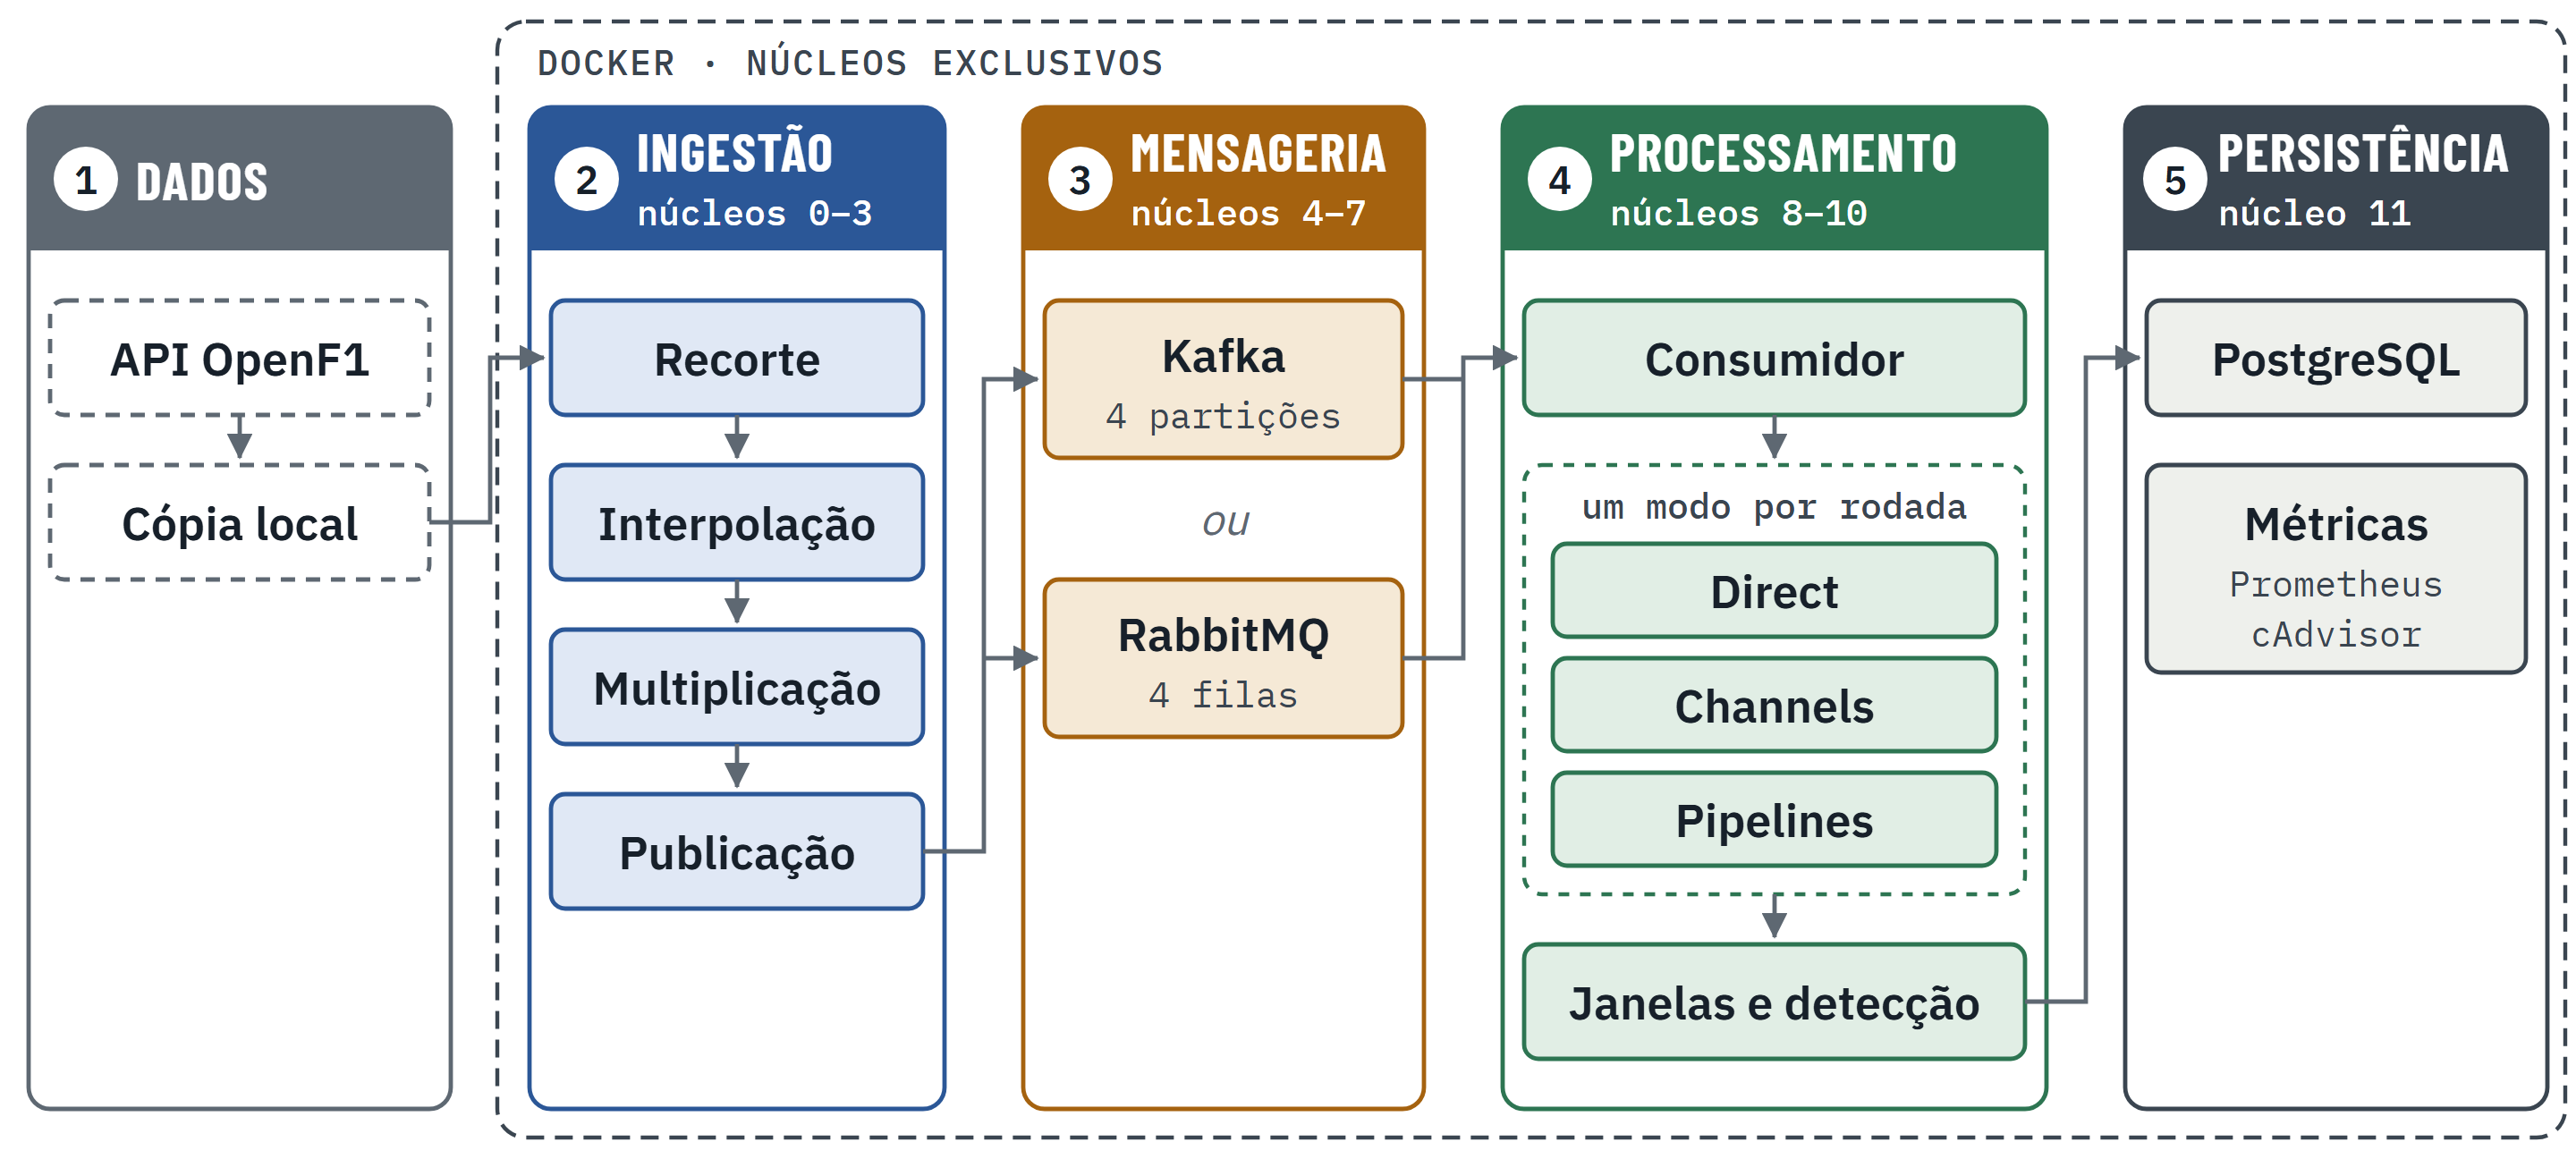
\includegraphics[width=\textwidth]{arquitetura_geral.png}
\caption{Arquitetura da bancada experimental: do conjunto de dados da OpenF1 ao
consumidor e à persistência, com a coleta de métricas em todas as etapas.}
\label{fig:arquitetura_geral}
\end{figure}
% TODO: exportar a Figura 1 a partir do mapa da arquitetura (layout C).

O sistema é composto pelos seguintes módulos, conforme ilustrado na
Figura~\ref{fig:arquitetura_geral}:

\begin{itemize}
  \item \textbf{Ingestão}: baixa os dados históricos da OpenF1 uma única vez e os
        reproduz como carga, publicando no broker (Seção~\ref{sec:workload});
  \item \textbf{Mensageria}: RabbitMQ 4.3.6 ou Kafka 4.1.0, com quatro filas ou
        partições (Seção~\ref{sec:mensageria});
  \item \textbf{Processamento}: consumidor nos três modos, sobre a mesma biblioteca de
        processamento (Seção~\ref{sec:processamento});
  \item \textbf{Persistência}: grava em lote, num PostgreSQL 17, os resultados agregados;
  \item \textbf{Coleta de métricas}: latência por evento no consumidor, recursos de cada
        container e indicadores de validade da rodada (Seção~\ref{sec:coleta}).
\end{itemize}

Toda a infraestrutura é containerizada com Docker, e os containers de cada rodada são
criados e removidos por scripts, o que garante reprodutibilidade e padronização dos
experimentos.

\subsection{Carga de Trabalho}
\label{sec:workload}

A API da OpenF1 não é, por si só, uma fonte de alta frequência: a telemetria tem cerca
de 3,7~Hz por carro, o plano gratuito limita as requisições e os dados ao vivo exigem
assinatura. Por isso, os dados históricos são baixados uma vez para disco e reproduzidos
por um gerador próprio; a API não é chamada durante os experimentos.

\textbf{Multiplicação de frota.} Para obter 100 mil eventos por segundo de uma corrida
que produz cerca de 75, há duas opções: comprimir o tempo ou simular mais carros. A
segunda foi escolhida porque preserva o intervalo entre amostras de cada carro e
corresponde ao cenário de frota que motiva o trabalho. Cada réplica recebe número de
carro próprio e um deslocamento de fase, para que a frota não publique em rajadas
sincronizadas.

\textbf{Frequência de 100~Hz.} No cenário principal, cada carro é reamostrado de 3,7 para
100~Hz por interpolação, sobre um trecho da corrida que começa no décimo minuto.
Velocidade, rotação e acelerador são interpolados em linha reta; marcha, freio e DRS
permanecem em degrau, de modo que as frenagens e trocas de marcha detectadas são as mesmas
da corrida original, o que é verificado em teste. A 100 mil eventos por segundo, a carga
corresponde a uma frota de 1.000 carros. Uma bateria a 3,7~Hz, com os dados sem
interpolação, serve de análise de sensibilidade.

\textbf{Gerador em malha aberta.} O gerador emite cada evento no instante previsto pela
taxa alvo, independentemente das confirmações do broker, e registra o maior atraso entre
o instante previsto e o envio efetivo. Esse atraso é critério de validade da rodada
(Seção~\ref{sec:analise}).

\textbf{Formato da mensagem.} Cada evento é um registro binário de 46 bytes, de tamanho
fixo, com o número da sequência, a sessão, o carro, o instante da amostra, o instante da
publicação e os seis canais de telemetria. O formato binário evita que o custo de
interpretar texto domine a medição, e o tamanho fixo dispensa enquadramento no modo
Pipelines. A compressão fica desligada nos dois brokers, porque as réplicas de uma mesma
amostra têm conteúdo quase idêntico e favoreceriam artificialmente a compressão em lote do
Kafka.

\subsection{Mensageria}
\label{sec:mensageria}

Os dois brokers rodam com um único nó. A carga é dividida em quatro faixas: quatro
partições no Kafka e quatro filas clássicas no RabbitMQ. O carro de cada evento define
a faixa pela mesma função nos dois brokers (CRC32 da chave, a função padrão do cliente
do Kafka), de modo que os eventos de um carro chegam sempre em ordem e à mesma faixa. Do
lado do consumidor, há um consumidor por faixa nos dois brokers.

A garantia de entrega é \textit{at-least-once} nos dois: o produtor espera a confirmação
do broker (\texttt{acks=all} no Kafka, \textit{publisher confirms} no RabbitMQ), e o
consumidor confirma a mensagem só depois de entregá-la ao processamento. A configuração
completa está na Seção~\ref{sec:configuracao}.

\subsection{Processamento}
\label{sec:processamento}

A lógica de processamento é a mesma biblioteca nos três modos. Ela segue as operações de
referência dos benchmarks de processamento de fluxos \cite{arasu:2004,mutschler:2013}:

\begin{itemize}
  \item \textbf{agregação em janela por carro}: janelas de 1~s em tempo do evento, com
        velocidade média e máxima e contagem de eventos;
  \item \textbf{detecção de padrão sobre eventos consecutivos} do mesmo carro: frenagens
        (transição de freio solto para acionado) e trocas de marcha.
\end{itemize}

A detecção exige que os eventos de cada carro cheguem em ordem; se a ordem quebrar, as
contagens mudam. O resultado de cada rodada é resumido num \textit{digest} independente da
ordem de fechamento das janelas. Como todas as combinações processam a mesma entrada em
cada nível de carga, todas precisam produzir o mesmo digest: uma divergência indica perda
de evento, duplicação ou quebra de ordem.

Nos modos Channels e Pipelines, há um mecanismo e uma thread de trabalho por faixa. O canal
tem capacidade de 10.000 eventos, e o \texttt{Pipe} pausa o escritor com 460.000 bytes
pendentes (o mesmo volume, 10.000 eventos de 46 bytes) e o retoma na metade. Quando o
mecanismo enche, o consumidor espera, e a contrapressão chega ao broker, que deixa de
entregar novas mensagens.

\subsection{Persistência}

Os resultados das janelas são gravados no PostgreSQL em lote, por \texttt{COPY} binário,
em tabelas sem registro de transação (\texttt{UNLOGGED}) e com
\texttt{synchronous\_commit} desligado. O objetivo é que o banco não se torne o gargalo e
mascare as diferenças entre as combinações. A latência medida termina no fim do
processamento, antes da gravação, e a persistência é acompanhada à parte: uma rodada em
que a fila de gravação descarta janelas é inválida.

\subsection{Coleta de Métricas}
\label{sec:coleta}

\begin{itemize}
  \item \textbf{Latência}: o produtor grava na mensagem o instante da publicação, lido de um
        relógio monotônico; o consumidor compara esse valor com o mesmo relógio ao fim do
        processamento. Como produtor e consumidor rodam na mesma máquina, os relógios são
        comparáveis sem sincronização. As latências são registradas em histogramas
        HdrHistogram, que preservam a cauda da distribuição;
  \item \textbf{Throughput}: eventos processados por segundo na janela de medição;
  \item \textbf{CPU e memória} de cada container, pelo cAdvisor, coletadas pelo Prometheus;
  \item \textbf{Alocações e coletas de lixo} do consumidor .NET, pelos contadores do
        runtime;
  \item \textbf{Validade}: atraso máximo de envio do gerador, digest do resultado,
        registros incompletos no \texttt{Pipe} e janelas descartadas na persistência;
  \item \textbf{Configuração efetiva}: os parâmetros de cada cliente e as variáveis de
        ambiente do .NET são gravados com cada rodada.
\end{itemize}

% ===================================================================

\section{Metodologia}
\label{sec:metodologia}

A pesquisa adota uma abordagem experimental de natureza quantitativa \cite{jain:1991}.
O protocolo foi definido em duas etapas: uma calibração, com medições exploratórias que
levaram a correções no ambiente e na configuração (Seção~\ref{sec:calibracao}), e a
coleta oficial, com o cenário congelado e a análise registrada antes de ver os dados.

\subsection{Ambiente}

Os experimentos foram executados num computador com processador Intel Core i5-12400F
(6 núcleos e 12 threads) e 16~GB de memória, com Windows~11 e Docker Desktop sobre WSL2,
cuja máquina virtual tem 12 núcleos lógicos e 8~GB de memória. Todos os componentes rodam
em containers, e cada um tem núcleos exclusivos: gerador nos núcleos 0 a 3, broker nos
núcleos 4 a 7, consumidor nos núcleos 8 a 10, e banco de dados e coleta de métricas no
núcleo 11. Os brokers têm o mesmo limite de 3~GB de memória. Durante as medições, só o
broker medido fica em execução, os painéis de visualização ficam desligados e o computador
não é usado.

\subsection{Configuração dos Brokers}
\label{sec:configuracao}

A comparação usa dois cenários de configuração. O \textbf{cenário padrão} usa os valores
de fábrica dos brokers e das bibliotecas cliente, exceto onde eles impedem a equivalência
entre os brokers; é a linha de base. O \textbf{cenário ajustado} aplica a recomendação de
cada fornecedor para vazão e latência \pendente{definir o perfil ajustado depois da
matriz do cenário padrão}. Os valores de fábrica foram conferidos na fonte de cada
versão, e não na documentação genérica. A Tabela~\ref{tab:configuracao} lista o que difere
do valor de fábrica no cenário padrão.

\begin{table}[ht]
\centering
\caption{Configuração do cenário padrão: parâmetros fora do valor de fábrica e o motivo.}
\label{tab:configuracao}
\small
\begin{tabular}{|p{2.6cm}|p{4.6cm}|p{6.4cm}|}
\hline
\textbf{Componente} & \textbf{Parâmetro e valor} & \textbf{Motivo} \\
\hline
Ambos & 4 faixas, carro por CRC32 & ordem por carro e mesma divisão nos dois brokers \\
\hline
Ambos & compressão desligada & a repetição do conteúdo favoreceria o Kafka \\
\hline
Ambos & até 100 mil mensagens sem confirmação no produtor & limites equivalentes; é o valor de fábrica do Kafka \\
\hline
Kafka, produtor & \texttt{acks=all}, sem idempotência & \textit{at-least-once}, como no RabbitMQ \\
\hline
Kafka, consumidor & offset guardado só depois do processamento & \textit{at-least-once} \\
\hline
Kafka, broker & 1 nó, replicação 1; retenção de 15 min & máquina única; só espaço em disco \\
\hline
RabbitMQ, produtor & \textit{publisher confirms} em lotes de 12.500, dois em voo por faixa; mensagem persistente & equivalente ao \texttt{acks=all}; mesmo total do Kafka \\
\hline
RabbitMQ, produtor & uma conexão por faixa & recomendação do fornecedor para alta vazão \\
\hline
RabbitMQ, consumidor & confirmação em lotes de 100 & recomendação do fornecedor \\
\hline
RabbitMQ, servidor & memória considerada de 3~GB & o padrão calcula sobre a memória da máquina virtual, não do container \\
\hline
\end{tabular}
\end{table}

Uma diferença de garantia permanece e é declarada: com a mensagem persistente, o
RabbitMQ grava em disco antes de confirmar, enquanto o Kafka confirma com a mensagem no
cache do sistema operacional, o comportamento recomendado pelo próprio Kafka
\cite{kafka:docs}. Na calibração, essa gravação custou 48\% no P99 do RabbitMQ a 40 mil
eventos por segundo (Seção~\ref{sec:calibracao}).

\subsection{Protocolo Experimental}

\begin{itemize}
  \item \textbf{Fatores}: broker (2) $\times$ modo de processamento (3) $\times$ carga.
  \item \textbf{Cargas}: RabbitMQ em 10, 20, 40, 60 e 80 mil eventos por segundo; Kafka
        em 10, 20, 40, 60, 100, 200, 300 e 400 mil. As faixas saem de varreduras de
        saturação feitas na calibração, com pelo menos uma carga acima do ponto de
        saturação de cada broker.
  \item \textbf{Rodada}: 10~s de aquecimento, descartados, e 90~s de medição. A 50 mil
        eventos por segundo, 90~s somam 4,5 milhões de eventos, muito além do necessário
        para estimar o P99.
  \item \textbf{Repetições}: 10 por combinação de broker, modo e carga, em ordem sorteada
        dentro de cada broker, para que uma deriva do ambiente não recaia sobre uma só
        combinação.
  \item \textbf{Isolamento}: o tópico ou as filas são recriados a cada rodada, e os
        arquivos da rodada anterior são apagados antes do início.
  \item \textbf{Sensibilidade}: o modo direto a 3,7~Hz, sem interpolação, em duas cargas
        por broker, com 10 repetições.
\end{itemize}

No total, são 390 rodadas no cenário padrão, além de 40 de sensibilidade.

\subsection{Métricas de Avaliação}

\begin{itemize}
  \item \textbf{Latência}: percentis P50, P95 e P99 e máxima, do envio ao fim do
        processamento \cite{fu:2021};
  \item \textbf{Throughput}: número de eventos processados por segundo;
  \item \textbf{Ponto de saturação}: maior carga sustentada por cada combinação;
  \item \textbf{Uso de CPU}: do consumidor, do broker e do gerador;
  \item \textbf{Uso de memória}: pico do consumidor e do broker;
  \item \textbf{Custo do .NET}: bytes alocados por evento e coletas de lixo por milhão
        de eventos no consumidor.
\end{itemize}

\subsection{Validade das Rodadas e Análise}
\label{sec:analise}

As regras abaixo foram registradas no repositório antes da coleta oficial e não mudam
depois de ver os dados.

\textbf{Validade.} Uma rodada é inválida se o atraso máximo de envio do gerador passar de
50~ms, se o seu digest divergir do digest de referência da carga, se houver registro
incompleto no \texttt{Pipe} ou se a persistência descartar janelas. Rodadas inválidas
não são repetidas: contam como resultado no ponto de saturação.

\textbf{Descarte de discrepantes.} Dentro de cada combinação, sai a rodada cujo P99 fica
fora do intervalo $[Q_1 - 1{,}5\,\mathrm{IQR};\; Q_3 + 1{,}5\,\mathrm{IQR}]$, a regra de
Tukey \cite{tukey:1977}, aplicada uma única vez. O número de descartes é publicado.

\textbf{Resumo.} Cada combinação é resumida pela mediana e pelo desvio padrão das rodadas
válidas e não descartadas.

\textbf{Ponto de saturação.} Uma carga é sustentada quando a maioria das rodadas é válida,
a mediana do throughput chega a pelo menos 99\% da carga oferecida e a mediana do P99 fica
abaixo de 50~ms. O ponto de saturação é a maior carga sustentada com todas as menores
também sustentadas.

\textbf{Comparações.} O efeito do mecanismo interno é a diferença entre as medianas de
Channels ou Pipelines e a do modo direto, no mesmo broker e carga. Diferenças abaixo de
10\% no throughput ou de 20\% no P99 são reportadas como sem diferença relevante. O teste
de Kruskal-Wallis \cite{kruskal:1952}, com nível de 5\%, acompanha as diferenças acima
desse tamanho, mas não sustenta conclusão sozinho.

\subsection{Calibração do Protocolo}
\label{sec:calibracao}

Antes da coleta oficial, três baterias de medições exploratórias (uma primeira matriz com
165 rodadas, um experimento fatorial 2$\times$2 e varreduras de saturação) mostraram
efeitos do ambiente que teriam sido atribuídos às arquiteturas:

\begin{itemize}
  \item \textbf{Clientes fora dos containers.} Com o gerador e o consumidor no Windows, o
        Kafka tinha latência bimodal em cerca de 43\% das rodadas de carga baixa. Com os
        mesmos programas em containers, o efeito desapareceu, e esse passou a ser o
        arranjo do protocolo.
  \item \textbf{Cota de CPU.} Com limites de CPU por cota, o broker RabbitMQ era
        estrangulado em 4 a 8\% dos períodos de escalonamento. Com núcleos exclusivos, o
        P99 do RabbitMQ caiu de 40\% a 64\%.
  \item \textbf{Auditoria da configuração.} A comparação com os valores de fábrica
        encontrou três defeitos de configuração (o algoritmo de Nagle ligado só no Kafka,
        o limite de memória do RabbitMQ calculado sobre a máquina virtual e o log do Kafka
        gravado na camada do container) e três assimetrias entre os brokers, todos
        corrigidos ou decididos com medições antes da coleta oficial.
  \item \textbf{Gravação de disco da máquina virtual.} A partir de 100 mil eventos por
        segundo, o Kafka teve episódios de 200~ms a 2~s sem confirmar nem entregar. A
        investigação, com uma linha do tempo de 100~ms por rodada, mostrou que eles
        coincidem com a gravação periódica em lote das páginas escritas pelo Kafka no
        disco virtual: logo depois de uma parada da máquina virtual por espera de disco, a
        chance de a latência passar de 50~ms foi 126 vezes maior. Os episódios ocorreram
        com e sem o Channels e não foram causados pelas coletas de lixo do .NET ou do
        broker.
\end{itemize}

Os resultados dessa etapa servem apenas de calibração e não entram na análise.

% ===================================================================

\section{Resultados e Discussão}
\label{sec:resultados}

% Estrutura prevista (ANALISE.md, seção 7). Os números saem da matriz v3.
% O orientador pediu a explicação de cada resultado: por que um broker foi
% mais rápido, se tem a ver com a carga, por quê. Cada subseção termina com
% a explicação, apoiada nas medições de recursos e na calibração.

\subsection{Validade das Rodadas}

\pendente{Tabela com rodadas totais, válidas, inválidas por motivo e descartadas por Tukey,
por combinação. Digest idêntico entre as seis combinações em cada carga.}

\subsection{Throughput e Ponto de Saturação}

\pendente{Tabela dos pontos de saturação por combinação. Figura: throughput entregue por
carga oferecida.}

% Pontos a explicar:
% - por que o Kafka satura numa carga maior: envio em lote por partição,
%   leitura sequencial do log e confirmação sem gravar em disco;
% - por que o RabbitMQ satura antes: roteamento e confirmação por mensagem,
%   gravação em disco antes de confirmar (custo medido na calibração), CPU do
%   broker perto do limite dos 4 núcleos (ensaio: cerca de 300%);
% - o que limita cada combinação na saturação: broker, consumidor ou gerador.

\subsection{Latência}

\pendente{Figura: P99 por carga, uma linha por modo, um painel por broker. Tabela de P50,
P95 e P99 nas cargas comuns aos dois brokers.}

% Pontos a explicar:
% - comparação dos brokers nas cargas comuns (10 a 80 mil);
% - dispersão maior do Kafka a partir de 100 mil, pelos episódios de
%   gravação do disco virtual (Seção de calibração e ameaças);
% - sensibilidade: 3,7 Hz contra 100 Hz.

\subsection{Efeito do Mecanismo Interno}

\pendente{Diferença de Channels e Pipelines para o modo direto em latência e CPU do
consumidor, por broker e carga, com o tamanho de efeito.}

% Pontos a explicar (a calibração indicou, a confirmar com a matriz):
% - com processamento leve, o mecanismo interno não reduz a latência e custa
%   CPU, cerca de 3,6 µs por evento, a ordem de grandeza de acordar uma
%   thread a cada evento;
% - o desacoplamento compensa quando há espera a esconder, o que não ocorre
%   quando o processamento custa cerca de 0,12 µs por evento;
% - Channels e Pipelines: objetos contra bytes, alocações por evento.

\subsection{Custo de Recursos no .NET}

\pendente{Figura: CPU do consumidor por mil eventos por segundo, por modo. Figura: bytes
alocados e coletas de lixo por evento, por modo.}

\subsection{Cenário Ajustado}

\pendente{Comparação do cenário ajustado com o padrão, depois da fase 7.}

% Se o segundo cenário (republicação) for aprovado e medido, entra aqui como
% subseção própria.

% ===================================================================

\section{Ameaças à Validade}
\label{sec:ameacas}

\subsection{Validade Interna}

\textbf{Máquina única e virtualizada.} Gerador, broker, consumidor e banco rodam no mesmo
computador, em containers sobre a máquina virtual do WSL2. Isso torna a medição de
latência válida sem sincronizar relógios, mas não exercita replicação, tolerância a falhas
nem rede entre máquinas, que são parte do que justifica o Kafka. As conclusões valem para
implantação de nó único. A mitigação são os núcleos exclusivos, os limites fixos de
memória, a ordem sorteada das rodadas e a documentação do ambiente.

\textbf{Gravação de disco da máquina virtual.} A gravação periódica em lote das páginas
escritas pelo Kafka para o disco virtual causa episódios de latência alta a partir de 100
mil eventos por segundo (Seção~\ref{sec:calibracao}). É o comportamento do Kafka sobre
este disco, que não força a gravação e conta com o cache do sistema operacional. Ajustar
a gravação do sistema operacional fugiria do cenário padrão e mudaria o ambiente dos dois
brokers; a mitigação são as dez repetições, a mediana e a regra de descarte, que impedem
um episódio isolado de decidir o ponto de saturação.

\textbf{Assimetria de durabilidade.} Com a mensagem persistente, o RabbitMQ oferece
garantia mais forte que o Kafka em nó único, o que favorece o Kafka. Equalizar exigiria
mensagens transitórias no RabbitMQ ou gravação forçada no Kafka, as duas fora da prática
recomendada de cada fornecedor. O custo foi medido e é declarado.

\textbf{Ordem por carro.} Para garantir a ordem dos eventos de cada carro nos dois
brokers, o RabbitMQ usa uma fila por faixa, em vez de uma fila com consumidores
concorrentes. Com isso, ele fica exposto ao bloqueio na cabeça da fila, como o Kafka por
partição.

\textbf{Omissão coordenada.} Um gerador que desacelera sob saturação deixaria de
registrar as latências altas. O gerador em malha aberta e o critério de atraso máximo de
envio cobrem esse risco.

\textbf{Observação.} A coleta de métricas (Prometheus e cAdvisor) roda durante todas as
rodadas, com os mesmos recursos em todas as combinações; os painéis de visualização
ficam desligados.

\subsection{Validade de Construto}

\textbf{Carga interpolada.} A OpenF1 fornece 3,7~Hz por carro, enquanto um carro de
Fórmula~1 tem sensores amostrados até 100~Hz. Os pontos intermediários a 100~Hz são
interpolados, e não medidos. Para os brokers, o conteúdo não importa, porque o evento tem
46 bytes de qualquer forma; para o processamento, as frenagens e trocas de marcha são as
mesmas da corrida original. O que muda é a forma da carga: menos carros distintos e mais
eventos por carro. A bateria a 3,7~Hz mostra o que depende da frequência.

\textbf{Conteúdo repetitivo.} As réplicas da frota têm conteúdo quase idêntico, o que
favoreceria a compressão em lote. Por isso a compressão foi desligada nos dois brokers;
em produção, o Kafka costuma usar compressão.

\textbf{Mensagem pequena e processamento leve.} Com eventos de 46 bytes e processamento de
cerca de 0,12~µs por evento, o experimento é dominado pelo transporte. Os resultados sobre
o mecanismo interno valem para esse uso; mensagens maiores ou processamento mais pesado
podem favorecer o Channels ou o Pipelines.

\subsection{Validade de Conclusão}

\textbf{Variância entre execuções.} Na calibração, a mesma configuração chegou a variar
três ordens de grandeza no P99 entre rodadas sucessivas. Uma rodada isolada não sustenta
conclusão neste ambiente; por isso as dez repetições, a regra de descarte fixada antes
da coleta e a análise por mediana.

\textbf{Significância e relevância.} Com dispersão pequena, diferenças irrelevantes
podem ser estatisticamente significativas. O tamanho de efeito relevante foi fixado
antes da coleta, e o teste estatístico só acompanha diferenças acima dele.

\subsection{Validade Externa}

Os resultados valem para as versões avaliadas (Kafka 4.1.0, RabbitMQ 4.3.6 com filas
clássicas, .NET 10), para um nó de cada broker e para o hardware descrito. Outros tipos de
fila do RabbitMQ, como as filas de quórum e os \textit{streams}, não foram avaliados.

% ===================================================================

\section{Considerações Finais}
\label{sec:conclusao}

Este trabalho avaliou experimentalmente arquiteturas compostas de processamento de eventos
em alta frequência utilizando .NET, combinando sistemas de mensageria distribuída
(RabbitMQ e Kafka) com mecanismos de processamento concorrente interno (Channels e
Pipelines), com um modo sem mecanismo interno como grupo de controle.

\pendente{Síntese dos resultados: pontos de saturação, efeito do mecanismo interno, custo
de recursos e recomendação prática para a escolha da arquitetura.}

Do ponto de vista metodológico, a calibração mostrou que, neste tipo de ambiente,
efeitos de virtualização, de limitação de CPU e de configuração podem ser maiores que a
diferença entre as arquiteturas. Uma comparação justa exigiu núcleos exclusivos,
configurações auditadas contra os valores de fábrica, repetições e critérios de análise
registrados antes da coleta.

Como trabalhos futuros, ficam: a avaliação em vários nós, com replicação; as filas de
quórum e os \textit{streams} do RabbitMQ; mensagens maiores e compressão; e um cenário
em que o consumidor republica o resultado em outro tópico, com garantia de ponta a ponta,
no qual o mecanismo interno tem espera de broker a esconder \pendente{remover se o segundo
cenário for incluído no trabalho}.

% ===================================================================

\bibliographystyle{sbc}
\bibliography{sbc-template}

\end{document}
